\section{Einleitung}
%Kontext
In Zusammenarbeit mit dem Spezialisten für Konserventechnik, der Ferrum AG, ist die Fachhochschule Nordwestschweiz FHNW daran, einen neuen Dosenverschliesser für die Getränke- und Lebensmittelindustrie zu entwickeln. Dieser soll hauptsächlich kleinere Unternehmen ansprechen mit begrenztem Budget und geringeren Anforderungen hinsichtlich des Durchsatzes. Die Maschine besteht aus vier Motoren inklusive dazugehöriger Werkzeuge, angeordnet auf einem Drehteller. Diese führen nacheinander die notwendigen Arbeitsschritte aus, um eine Dose zu verschliessen. Das Institut für Automation der FHNW hat bereits einen ersten Aufbau der Maschine realisiert. Dabei werden die vier Motoren-Drives mit einer Schleppkette versorgt, welche die Kabel für Energieversorgung und Datenkommunikation führt. Eine Schleppkette ist wartungsintensiv und sperrig und deshalb für eine industrielle Anlage ungeeignet.
\newline
\ \\
%Ziel+Anforderungen
In dieser Projektarbeit soll deshalb eine berührungslose Energie- und Datenübertragung auf den Drehteller realisiert werden. Das heisst, die Kabel und die lange Schleppkette sollen ganz ersetzt werden. Die vier Motoren brauchen zusammen eine Leistung von mindestens $\SI{300}{W}/\SI{48}{V}$. Das heisst, diese Leistung muss berührungslos übertragen werden können. Die Datenübertragung funktioniert über einen VARAN-Ethernet-Bus. Dieser wird mit einer Frequenz von \SI{31.25}{MHz} betrieben. Ziel im Projekt 5 ist es, mit Simulationen und Testaufbauten möglichst viele Erkenntnisse zur berührungslosen Energie- und Datenübertragung zu sammeln um daraus ein Konzept zu erarbeiten. Mit diesem, im Projekt 5 ausgearbeiteten Konzept, wird die Vorarbeit für die Bachelor-Thesis geleistet. Dort soll schliesslich ein Produkt entstehen, welches im Dosenverschliesser die Schleppkette ersetzen kann.
\newline
\ \\
%Lösungsansätze
Die Bedingungen und genauen Spezifikationen der drahtlosen Übertragung sowohl der Energie als auch der Daten werden mit ausgedehnten Simulationen ermittelt. Die Energieübertragung basiert auf Induktion. Hierfür sind zwei Spulen mit Kern realisiert, sie müssen dimensioniert und die Ansteuerung mit gängigen Testschaltungen eruiert werden. Die Daten dagegen sollen via optischer Übertragung auf den Drehteller und zurück gesendet werden. Dafür sind Infrarot-Emitter, Photodioden und Transimpedanzverstärker zu evaluieren und zu simulieren. Für eine störungsarme Übertragung sind zwei optisch getrennte Kanäle vorgesehen. Ob die Geschwindigkeit der Übertragung genügend schnell, störungsfrei und sicher ist, soll mit einer eigens gebauten Testschaltung geprüft werden.
\newline
\ \\ 
%Aufbau der Arbeit
Die Energieübertragung und die Datenübertragung sind im Projekt 5 separat untersucht worden. Entsprechend sind die beiden Themen im vorliegenden Bericht auch getrennt dargelegt. Im Kapitel \ref{sec:Grundlagen} \nameref{sec:Grundlagen} sind die wichtigsten Theorien und Erklärungen sowohl für die Daten- als auch für die Energieübertragung erläutert. Die \nameref{sec:energie} selbst wird im Kapitel \ref{sec:energie} vom Konzept bis zur Validierung des Testaufbaus detailliert dargelegt, im Kapitel \ref{sec:Daten} \nameref{sec:Daten} dasselbe für die Sende- und Empfängerschaltung. Das Kapitel \ref{sec:Schlussbemerkung} \nameref{sec:Schlussbemerkung} schliesslich fasst die wichtigsten Erkenntnisse zusammen und beschreibt die Ausgangslage für das Projekt 6.


%\begin{figure}
%\centering
%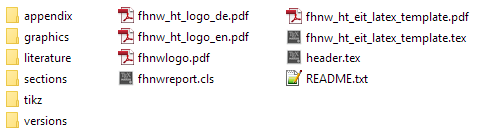
\includegraphics[width=0.8\linewidth]{ordner_struktur.png}
%\caption{Minimalstruktur des \LaTeX -Projekts.}\label{fig:Struktur}
%\end{figure}

